%%%%%%%%%%%%%%%%%%%%%%%%%%%%%%%%%%%%%%%%%%%%%%%%%%%%%%%%%%%%%%%
%
% Welcome to Overleaf --- just edit your LaTeX on the left,
% and we'll compile it for you on the right. If you open the
% 'Share' menu, you can invite other users to edit at the same
% time. See www.overleaf.com/learn for more info. Enjoy!
%
%%%%%%%%%%%%%%%%%%%%%%%%%%%%%%%%%%%%%%%%%%%%%%%%%%%%%%%%%%%%%%%
\documentclass{beamer}
 \usetheme[options]{Boadilla}
 % paquets pour le français
 \usepackage{tikz}
 \usepackage{multicol}
 \usepackage[T1]{fontenc}
 \usepackage[utf8]{inputenc}
\usepackage{minted}
\definecolor{LightGray}{gray}{0.9}
  \title{Programmation C: Fonction}
  \author{ \textsc{Ibrahim ALAME}}\institute{ESIEE}
\date{27/11/2023}
\begin{document}
\maketitle
 \begin{frame}
  \frametitle{Fonctions}
  \begin{block}{Définition}
 Une fonction est une suite d'instructions, mais vue du programme principal {\bf main()}, elle représente une seule action.
Deux types de fonction:
\begin{itemize}
\item Les fonctions prédéfinies  {\bf scanf, printf, strcpy}…
\item les fonctions personnelles
\end{itemize}
\end{block}

Utilité des fonctions:
\begin{itemize}
\item Supprimer les répétitions de code
\item Structurer des blocs de code indépendants (maintenance)
\item Création de bibliothèques de fonctions
\end{itemize}

  \end{frame}
  
\begin{frame}[fragile]
\frametitle{Quelques exemples}
Une définition de fonction spécifie :
\begin{itemize}
\item Le type de la valeur renvoyée par la fonction
\item Le nom de la fonction
\item Les paramètres (argument) qui sont passés à la fonction
\item Les variables locales et externes utilisées par la fonction
\item D'autre fonctions appelées éventuellement par la fonction
\item Les instructions que doit exécuter la fonction
\end{itemize}

\underline {\em Syntaxe d'une fonction:}

\begin{minted}[
%frame=lines,
framesep=2mm,
baselinestretch=1.2,
bgcolor=LightGray,
fontsize=\footnotesize,
% linenos
]{c}
<type_iden_sortie> iden_Fct( <type> ien_1, ... ,<type> iden_N){
        /* déclaration  des variables locales */
        <type>  iden_2,...,iden_Z;
        //
        // Traitement 
        //
        /* renvoi le résultat dans le paramètre de sortie*/
        return(valeur);
    }

\end{minted}

\end{frame}
  
  
 
%%%%%%%%%%%%%%%%%%%%%%%%%%%%%%%%%%%%%%%%%%%%%%%%%%%%%%%%%%%%%%%
\begin{frame}[fragile]
\frametitle{Quelques exemples}
\underline {\em Exemple d'une fonction:}
\begin{minted}[
%frame=lines,
framesep=2mm,
baselinestretch=1.2,
bgcolor=LightGray,
fontsize=\footnotesize,
% linenos
]{c}
    double carre (double C ) {      
        double resultat;   /* déclaration  d'une variable locale */
        resultat = C * C;
        /* renvoi le résultat dans le paramètre de sortie*/
        return (resultat);
    }
\end{minted}
    Autres caractéristiques des fonctions :
\begin{itemize}
\item Une fonction peut en appeler une autre. La fonction appelée doit être déclarée avant celle qui appelle.
\item On ne peut pas déclarer une fonction à l'intérieur d'une autre fonction.
\item Une fonction possède un seul point d'entrée, mais éventuellement plusieurs de sortie. 
\end{itemize}

\end{frame}
  
  
 
%%%%%%%%%%%%%%%%%%%%%%%%%%%%%%%%%%%%%%%%%%%%%%%%%%%%%%%%%%%%%%%

\begin{frame}[fragile]
\frametitle{Où déclarer  une fonction? : avant le main()}
\begin{minted}[
%frame=lines,
framesep=2mm,
baselinestretch=1.2,
bgcolor=LightGray,
fontsize=\footnotesize,
% linenos
]{c}
#include <stdio.h>

double carre (double C ) {      
    double resultat; // déclaration  d'une variable locale
    resultat = C * C;
    return( resultat ); // renvoi le résultat à la sortie
    }
    
int main(){
 	double A, B=2;
  	A = carre (B );
 	printf ("Le carré de %f est %f",B,A);
    return 0;
}
\end{minted}
\end{frame}
%%%%%%%%%%%%%%%%%%%%%%%%%%%%%%%%%%%%%%%%%%%%%%%%%%%%%%%%%%%%%%%%%

\begin{frame}[fragile]
\frametitle{Où déclarer  une fonction? : après le main()}
\begin{minted}[
%frame=lines,
framesep=2mm,
baselinestretch=1.2,
bgcolor=LightGray,
fontsize=\footnotesize,
% linenos
]{c}
#include <stdio.h>

double carre (double C ) ; // PROTOTYPE DE LA FONCTION

int main(){
 	double A, B=2;
  	A = carre (B );
 	printf ("Le carré de %f est %f",B,A);
    return 0;
}

double carre (double C ) {      
    double resultat; // déclaration  d'une  variable locale
    resultat = C * C;
    return( resultat ); // renvoi le résultat à la sortie
}

\end{minted}
\end{frame}
%%%%%%%%%%%%%%%%%%%%%%%%%%%%%%%%%%%%%%%%%%%%%%%%%%%%%%%%%%%%%%%%%



\begin{frame}[fragile]
\frametitle{Déclaration PROTOTYPE}
Le prototype de la fonction définie l'interface de la fonction. Lors de la compilation, le compilateur accepte l'appel à une fonction seulement s'il à rencontré au moins le prototype de la fonction. Dans la déclaration prototype il est possible d'omettre les noms des variables mais pas leur type.

\begin{minted}[
%frame=lines,
framesep=2mm,
baselinestretch=1.2,
bgcolor=LightGray,
fontsize=\footnotesize,
% linenos
]{c}
#include <stdio.h>
double carre (double) ; // PROTOTYPE SANS NOM DE VARIABLE
int main(){
 	double A, B=2;
  	A = carre (B );
 	printf ("Le carré de %f est %f",B,A);
    return 0;
}
double carre (double C ) {      
    double resultat; // déclaration  d'une  variable locale
    resultat = C * C;
    return( resultat ); // renvoi le résultat à la sortie
}

\end{minted}
\end{frame}
%%%%%%%%%%%%%%%%%%%%%%%%%%%%%%%%%%%%%%%%%%%%%%%%%%%%%%%%%%%%%%%%%


\begin{frame}[fragile]
\frametitle{Les fonctions et les échanges de variables }
\underline {\em Deux types:}

\begin{itemize}
\item Les fonctions sans passage de paramètres et ne renvoyant rien au programme :    
		
\begin{minted}[
%frame=lines,
framesep=2mm,
baselinestretch=1.2,
bgcolor=LightGray,
fontsize=\footnotesize,
% linenos
]{c}
void UneFonction ( void ); 
\end{minted}
\item Les fonctions avec passage de paramètres et renvoyant un objet au programme :
		
\begin{minted}[
%frame=lines,
framesep=2mm,
baselinestretch=1.2,
bgcolor=LightGray,
fontsize=\footnotesize,
% linenos
]{c}
int UneFonction ( int A ): 
\end{minted} 

\end{itemize}


\end{frame}
%%%%%%%%%%%%%%%%%%%%%%%%%%%%%%%%%%%%%%%%%%%%%%%%%%%%%%%%%%%%%%%%%


\begin{frame}[fragile]
\frametitle{Les fonctions et les échanges de paramètres : Par des variables globales}

    Une variable globale est déclarée au début du programme.
    Cette variable sera visible dans toutes les fonctions

    \underline {\em Exemple}
	
\begin{minted}[
%frame=lines,
framesep=2mm,
baselinestretch=1.2,
bgcolor=LightGray,
fontsize=\footnotesize,
% linenos
]{c}
#include <stdio.h>

int X; /* déclaration de X en variable globale */

void main() {
...

}
\end{minted}

\end{frame}
%%%%%%%%%%%%%%%%%%%%%%%%%%%%%%%%%%%%%%%%%%%%%%%%%%%%%%%%%%%%%%%%%



\begin{frame}[fragile]
\frametitle{Les fonctions et les échanges de paramètres : Par des variables locales}
\begin{itemize}
\item Une variable locale est déclarée au début d'une fonction.
\item Cette variable sera visible uniquement dans la fonction.
\item Une variable globale portant le même nom sera invisible dans la fonction.
\item Les variables locales ne sont pas initialisées par défaut et perdent leur valeur à chaque nouvel appel de la fonction
\end{itemize}

\begin{minted}[
%frame=lines,
framesep=2mm,
baselinestretch=1.2,
bgcolor=LightGray,
fontsize=\footnotesize,
% linenos
]{c}
#include <stdio.h>
int X,A;  /* déclaration de X et A en variable globale */
int MaFonction( int A) {  /* déclaration de A en variable locale */ 
    static int X;         /* déclaration de X en variable locale */
	. . .
    return (X);
}
void main(void) {
	. . .
}
\end{minted}

\end{frame}
%%%%%%%%%%%%%%%%%%%%%%%%%%%%%%%%%%%%%%%%%%%%%%%%%%%%%%%%%%%%%%%%%

\begin{frame}[fragile]
\frametitle{Échange entre les fonctions par variables globales}

\begin{minted}[
%frame=lines,
framesep=2mm,
baselinestretch=1.2,
bgcolor=LightGray,
fontsize=\footnotesize,
% linenos
]{c}
#include <stdio.h>                         

int A,B;
void cube(void);

int main(void) {
    A=2; // initialisation de A à 2
    int B; /* déclaration locale de B */
    printf("A=%d, B=%d\n",A,B);	/* affiche : A=4, B=0  */
    cube();
    printf("A=%d, B=%d\n",A,B);	/* affiche : A=4, B=0   */	
}

void cube() { 	
    B = A*A*A;
    return;
}
\end{minted}

\end{frame}
%%%%%%%%%%%%%%%%%%%%%%%%%%%%%%%%%%%%%%%%%%%%%%%%%%%%%%%%%%%%%%%%%

\begin{frame}[fragile]
\frametitle{Échange entre les fonctions par variables locales}

\begin{minted}[
%frame=lines,
framesep=2mm,
baselinestretch=1.2,
bgcolor=LightGray,
fontsize=\footnotesize,
% linenos
]{c}
#include <stdio.h> 

int cube(int);

int main(void) {
    int A=2; //déclaration locale et initialisation de A à 2
    int B; /* déclaration locale de B */
    printf("A=%d, B=%d\n",A,B);	/* affiche : A=4, B=??   */
    B = cube(A);
    printf("A=%d, B=%d\n",A,B);	/* affiche : A=4, B=8   */	
}

int cube(int X) { /* X est un paramètre de la fonction cube */
              /* X récupère la valeur de A du main */
	int resultat;		
    resultat = X*X*X;
    return (resultat);
}
\end{minted}

\end{frame}
%%%%%%%%%%%%%%%%%%%%%%%%%%%%%%%%%%%%%%%%%%%%%%%%%%%%%%%%%%%%%%%%%

\begin{frame}[fragile]
\frametitle{Échange entre les fonctions par variables locales}

\begin{minted}[
%frame=lines,
framesep=2mm,
baselinestretch=1.2,
bgcolor=LightGray,
fontsize=\footnotesize,
% linenos
]{c}
#include <stdio.h> 
void cube(int);
int main(void) {
    int A=2; //déclaration locale et initialisation de A à 2
    int B; /* déclaration locale de B */
    printf("A=%d, B=%d\n",A,B);	/* affiche : A=4, B=??   */
    cube(A);
    printf("A=%d, B=%d\n",A,B);	/* affiche : A=4, B=??   */	
}

void cube(int A) { /* A est un paramètre de la fonction cube */
			/* A récupère la valeur de A du main */
	int B;		
	B = A*A*A;
	printf("A=%d, B=%d\n",A,B);	/* affiche : A=4, B=8   */	
	return ;
}
\end{minted}

\end{frame}
%%%%%%%%%%%%%%%%%%%%%%%%%%%%%%%%%%%%%%%%%%%%%%%%%%%%%%%%%%%%%%%%%

\begin{frame}[fragile]
\frametitle{Échange entre les fonctions par variables locales}

\begin{minted}[
%frame=lines,
framesep=2mm,
baselinestretch=1.2,
bgcolor=LightGray,
fontsize=\footnotesize,
% linenos
]{c}
#include <stdio.h>                         
void cube(int, int*);
int main(void) {
    int A=2; /* déclaration locale de A et B */
    int B;
    printf("A=%d, B=%d\n",A,B);/* affiche : A=4, B=??   */
    cube( A , &B);//On donne à la fonction cube le contenu de A 
                  // et l'adresse de de la variable B
    printf("A=%d, B=%d\n",A,B);/* affiche : A=4, B=??   */	
}

void cube(int A, int *B) {/* A est un paramètre de la fonction*/
		/* B récupère un pointeur sur un entier */
    printf("> A=%d, B=%d\n",A,*B);/* affiche : A=4, B=??   */
    *B = A*A*A;
    printf("> A=%d, B=%d\n",A,*B);/* affiche : A=4, B=8   */
    return;
}

\end{minted}

\end{frame}
%%%%%%%%%%%%%%%%%%%%%%%%%%%%%%%%%%%%%%%%%%%%%%%%%%%%%%%%%%%%%%%%%
\begin{frame}[fragile]
\frametitle{Fonction récursive }
\begin{itemize}
\item Une fonction récursive est une fonction qui s'appelle elle-même. 
\begin{itemize}
\item Directement (si la fonction $P$ appelle directement $P$ , on dit que la récursivité est directe). 
\begin{minted}[
%frame=lines,
framesep=2mm,
baselinestretch=1.2,
bgcolor=LightGray,
fontsize=\footnotesize,
% linenos
]{c}
int f1(...){
    x=f1(...);
    return ...;
}
\end{minted}
\item  Indirectement à travers une ou plusieurs fonctions relais (si $P$ appelle une fonction $P_1$ , qui appelle une fonction $P_2$ , ... , qui appelle une fonction $P_n$ et qui enfin appelle $P$ , on dit qu'il s'agit d'une récursivité indirecte).

\begin{minipage}[c]{0.48\linewidth}
\begin{minted}[
%frame=lines,
framesep=2mm,
baselinestretch=1.2,
bgcolor=LightGray,
fontsize=\footnotesize,
% linenos
]{c}
int f1(...){
    x=f2(...);
    return ...;
}
\end{minted}
\end{minipage}
\begin{minipage}[c]{0.48\linewidth}
    \begin{minted}[
%frame=lines,
framesep=2mm,
baselinestretch=1.2,
bgcolor=LightGray,
fontsize=\footnotesize,
% linenos
]{c}
int f2(...){
    x=f1(...);
    return ...;
}
\end{minted}
\end{minipage}
\end{itemize}
\end{itemize}
\end{frame}

%%%%%%%%%%%%%%%%%%%%%%%%%%%%%%%%%%%%%%%%%%%%%%%%%%%%%%%%%%%%%%%%%
\begin{frame}[fragile]
\frametitle{Fonction récursive }
\begin{itemize}
\item La récursivité est une manière simple et élégante de résoudre certains problèmes algorithmiques. 
\item Elle permet:
\begin{itemize}
\item  d'écrire des programmes beaucoup plus lisibles; 
\item d'écrire d'une manière très rapide (par rapport d'une manière itérative); 
\item d'utiliser le principe diviser-pour-résoudre.
\end{itemize}
\item  La récursivité utilise toujours la pile du programme en cours. 
\item  Dans une fonction récursive, toutes les variables locales sont stockées dans la pile, et empilées autant de fois qu'il y a d'appels récursifs. 
\item  La pile se remplit progressivement, et si on ne fait pas attention on arrive à un "débordement de pile". Ensuite, les variables sont désempilées. 
\item  Toute fonction récursive comporte une instruction (ou un bloc d'instructions) nommée "point terminal" ou "point d'appui" ou "point d'arrêt", qui indique que le reste des instructions ne doit plus être exécuté.
\end{itemize}
\end{frame}


%%%%%%%%%%%%%%%%%%%%%%%%%%%%%%%%%%%%%%%%%%%%%%%%%%%%%%%%%%%%%%%%%
\begin{frame}[fragile]
\frametitle{Fonction récursive : Syntaxe}
\begin{itemize}
\item La fonction récursive est composée de deux partie: une partie strictement récursive et une partie non récursive (base) servant de point de départ à l'utilisation de la définition récursive. 
\item Structure générale d'une fonction récursive : 
\end{itemize}
\begin{minted}[
%frame=lines,
framesep=2mm,
baselinestretch=1.2,
bgcolor=LightGray,
fontsize=\footnotesize,
% linenos
]{c}
if(/* !condition de convergence */) 
    exit(1); 
if(/*condition d’arrêt*/) 
    return(/*Ce qu’elle doit retourner*/); 
else 
/*Traitement*/
/*appel récursif */
/*Traitement*/
\end{minted}

\end{frame}

%%%%%%%%%%%%%%%%%%%%%%%%%%%%%%%%%%%%%%%%%%%%%%%%%%%%%%%%%%%%%%%%%
\begin{frame}[fragile]
\frametitle{Fonction récursive : Exemple}
 
\begin{itemize}
\item Soit le factoriel $n!=1\times 2\times 3 \cdots \times n$ pour $n$ entier naturel. Par convention $0!=1$.
\item Par récurrence le factoriel est calculé à l'aide de la suite récurrente:
\[\left\{\begin{array}{ll}
u_n=n\times u_{n-1} & \mbox{ pour } n\geq 1\\
u_0 =1&
\end{array}\right.
\]
\end{itemize}
\begin{minted}[
%frame=lines,
framesep=2mm,
baselinestretch=1.2,
bgcolor=LightGray,
fontsize=\footnotesize,
% linenos
]{c}
#include <stdio.h> 
#include <stdlib.h>
int u(int n){
    if(n<0) exit(EXIT_FAILURE);
    else
        if(n==0) return 1;
        else
            return n*u(n-1);
}
int main(void) {
    printf("n!=%d\n",u(5));	
}
\end{minted}

\end{frame}

%%%%%%%%%%%%%%%%%%%%%%%%%%%%%%%%%%%%%%%%%%%%%%%%%%%%%%%%%%%%%%%%%
\begin{frame}[fragile]
\frametitle{Fonction récursive : Variables locales, arguments de fonctions}
 
\begin{itemize}
\item Lorsqu'une fonction récursive définit des variables locales, un exemplaire de chacune d'entre elles est crée à chaque appel récursif de la fonction. 
\item Il en est de même des arguments des fonctions.
\item \underline {\em Exemple} - considérons une fonction {\bf void  miroir()} qui lit caractère par caractère une chaîne terminée par '?' et l'affiche dans l'ordre inverse de celui de la lecture.
\end{itemize}


\end{frame}


%%%%%%%%%%%%%%%%%%%%%%%%%%%%%%%%%%%%%%%%%%%%%%%%%%%%%%%%%%%%%%%%%
\begin{frame}[fragile]
\frametitle{Fonction itérative : Variables locales, arguments de fonctions}
 
\begin{minted}[
%frame=lines,
framesep=2mm,
baselinestretch=1.2,
bgcolor=LightGray,
fontsize=\footnotesize,
% linenos
]{c}
#include <stdio.h> 
void miroir() { 
    char s[20],c; 
    int i=0; 
    while( (c=getchar())!='?') 
        s[i++]=c; 
    s[i]='\0'; 
    while (--i>=0) 
        putchar (s[i]); 
}
void main() { 
    printf("Entrer les caracteres avec ? a la fin.\n"); 
    miroir(); 
    
}

\end{minted}

\end{frame}

%%%%%%%%%%%%%%%%%%%%%%%%%%%%%%%%%%%%%%%%%%%%%%%%%%%%%%%%%%%%%%%%%
\begin{frame}[fragile]
\frametitle{Fonction récursive : Variables locales, arguments de fonctions}
 
\begin{minted}[
%frame=lines,
framesep=2mm,
baselinestretch=1.2,
bgcolor=LightGray,
fontsize=\footnotesize,
% linenos
]{c}
#include <stdio.h> 
void miroir() { 
     int c = getchar(); 
     if (c != '?') { 
         miroir(); 
         printf("%c", c);        
     }    
 } 
 void main() { 
     printf("Entrer les caracteres avec ? a la fin.\n"); 
     miroir(); 
     
 }
\end{minted}

\end{frame}

%%%%%%%%%%%%%%%%%%%%%%%%%%%%%%%%%%%%%%%%%%%%%%%%%%%%%%%%%%%%%%%%%
\begin{frame}[fragile]
\frametitle{Fonction récursive : Variables locales, arguments de fonctions}
 
\begin{tabular}{|l|l|l|l|}\hline 
{\tt miroir() c='1'} & & & \\
\hline
 & {\tt miroir() c='2'} & & \\
\hline
& & {\tt miroir() c='3'} &  \\
\hline
& & & {\tt miroir() c='?'}   \\
\hline
& & & destruction de c  \\
& & & retour  \\
\hline
& & {\tt printf("\%c",c)}   &  \\
\hline 
& & destruction de c & \\
& & retour  & \\
\hline
& {\tt printf("\%c",c)}   &  &\\
\hline 
 & destruction de c & & \\
& retour  & &\\
\hline
 {\tt printf("\%c",c)}   & & &\\
\hline 
 destruction de c & & &\\
retour  & &&\\
\hline
\end{tabular}
\end{frame}

%%%%%%%%%%%%%%%%%%%%%%%%%%%%%%%%%%%%%%%%%%%%%%%%%%%%%%%%%%%%%%%%%
\begin{frame}[fragile]
\frametitle{Fonction récursive : Dangers et précautions}
 \begin{itemize}
\item Débordement de pile (Stack Overflow) 
\item Dans la pile sont non seulement stockés les valeurs des variables de retour mais aussi les adresses des fonctions entre autres choses, les données sont nombreuses et un débordement de la pile peut très vite arriver ce qui provoque sans conteste une sortie anormale du programme. 
\item Si vous êtes presque sûr de dépasser ce genre de limites, préférez alors une approche itérative plutôt qu'une approche récursive du problème.
 \end{itemize}
\end{frame}
%%%%%%%%%%%%%%%%%%%%%%%%%%%%%%%%%%%%%%%%%%%%%%%%%%%%%%%%%%%%%%%%%

\begin{frame}[fragile]
\frametitle{Fonction récursive ; Un piège subtil: la suite de Fibonacci}
 \begin{itemize}
\item Écrire une fonction qui calcule le $n$-ième terme de la suite définie par
\[\left\{\begin{array}{l}
F_0 = 0, F_1 = 1\\
F_n = F_{n-1} + F_{n-2}\quad\mbox{pour }n\geq 2
\end{array}\right.\]
\item Le programme marche, il termine. Le problème se situe dans le nombre exponentiel  d'appels à la fonction. 
 \end{itemize}
 
 \begin{minted}[
%frame=lines,
framesep=2mm,
baselinestretch=1.2,
bgcolor=LightGray,
fontsize=\footnotesize,
% linenos
]{c} 
#include <stdio.h> 
long fib(int n){ 
    if(n <= 1) 
        return n; // cas de base 
    else 
        return fib(n-1)+fib(n-2);  // cas général 
 } 
 void main() {
     int n=40;
     printf("fib(%d)=%ld\n",n,fib(n));  
 } 
\end{minted}

\end{frame}
%%%%%%%%%%%%%%%%%%%%%%%%%%%%%%%%%%%%%%%%%%%%%%%%%%%%%%%%%%%%%%%%%

\begin{frame}[fragile]
\frametitle{Fonction récursive ; Un piège subtil: la suite de Fibonacci}
 \begin{itemize}
\item Le programme marche, il termine. Le problème se situe dans le nombre exponentiel  d'appels à la fonction. 
 \end{itemize}
 
 
 \begin{center}
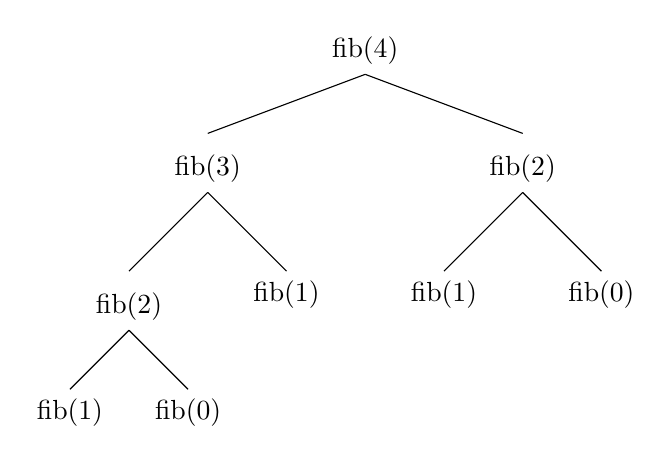
\begin{tikzpicture}[domain=-5:5,scale=0.50]
 %\pgfmathsetmacro{\alpha}{0.05}
 % \pgfmathsetmacro{\a}{0.8}
  %\draw[->] (0,0) -- (6*\a,0)  node[right] {$x$};
  %\draw[->] (0,0) -- (0,5.5*\a) node[left] {$y$};
\draw[-] (-4,6.5)--(0,8) node[above]{fib(4)};
\draw[-] (0,8)--(4,6.5) ;

\draw[-] (-6,3)--(-4,5) node[above]{fib(3)};
\draw[-] (-4,5)--(-2,3) node[below]{fib(1)};

\draw[-] (6,3)  node[below]{fib(0)}  --(4,5) node[above]{fib(2)};
\draw[-] (4,5)--(2,3) node[below]{fib(1)};

\draw[-] (-7.5,0)  node[below]{fib(1)}  --(-6,1.5) node[above]{fib(2)};
\draw[-] (-6,1.5)--(-4.5,0)  node[below]{fib(0)};
%  \foreach \n in {0,1,...,5}{
%   \draw[blue,thick](\n*\a,0)-- ++(0,5*\a);
%    \draw[blue,thick](0,\n*\a)-- ++(5*\a,0);
%}
%\draw (2*\a,0)  node[below] {$\scriptstyle  \ell h$};
%\draw (0,3*\a)  node[left] {$\scriptstyle  m h$};
%
%\draw[fill=orange!30] (2*\a,3*\a)  -- ++(\a,0) -- ++(0,\a) -- ++(-\a,0) -- ++(0,-\a);
%  \draw (2*\a,3.5*\a)  node[above,right] {$\scriptstyle  K_{l,m}$};
\end{tikzpicture}

\end{center}

\end{frame}


%%%%%%%%%%%%%%%%%%%%%%%%%%%%%%%%%%%%%%%%%%%%%%%%%%%%%%%%%%%%%%%%%

\begin{frame}[fragile]
\frametitle{Fonction récursive ; la suite de Fibonacci: version itérative}

\begin{minted}[
%frame=lines,
framesep=2mm,
baselinestretch=1.2,
bgcolor=LightGray,
fontsize=\footnotesize,
% linenos
]{c}  
#include <stdio.h> 
long fib(int n){ 
    int i;
    long u, v, w; 
    u = 0; v = 1; // u = F(0); v = F(1) 
    for(i = 2; i <= n; i++){ 
        w = u+v; // u = F(i-2); v = F(i-1) 
        u = v; 
        v = w; 
    } 
    return v;
}
void main() {
     int n=50;
     printf("fib(%d)=%ld\n",n,fib(n)); 
 }
\end{minted}

\end{frame}

%%%%%%%%%%%%%%%%%%%%%%%%%%%%%%%%%%%%%%%%%%%%%%%%%%%%%%%%%%%%%%%%%

\begin{frame}[fragile]
\frametitle{Fonction récursive ; Diviser pour résoudre}

\begin{itemize}
\item Quand on ne sait pas résoudre un problème, on essaie de le couper en morceaux qui seraient plus faciles à traiter. 
\item Exemple - Recherche d'une racine par dichotomie 
\item On suppose que $f :[a, b] \to \mathbb{R}$ est continue et telle que $f(a) < 0, f(b) > 0$. Il existe une racine $x_0$ de $f$ dans l'intervalle $[a, b]$, qu'on veut déterminer de sorte que $|f(x_0)| \leq \varepsilon$ pour $\varepsilon$ donné. On calcule $f(m)$ où $m=(a+b)/2$. En fonction de son signe, on explore $[a, m]$ ou $[m, b]$.
\end{itemize}

\begin{center}
 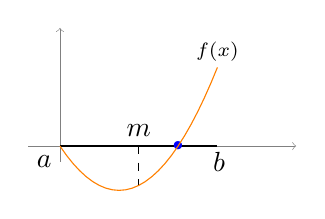
\begin{tikzpicture}[xscale=2]
\draw  [very thin, gray] [->]  (-0.2,0) -- (1.5,0); 
\draw  [very thin, gray] [->] (0,-0.2) -- (0,1.5);
\draw  [line width=1pt] (0,0) -- (1,0);
\draw  [dashed] (0.5,0) -- (0.5,-0.5);
\node [blue] at (0.75,0) {$\scriptstyle \bullet$};
\node at (1,1.2) {$\scriptstyle  f(x)$};
\draw [orange,domain=0:1] plot(\x,{4*\x*\x-3*\x});
\node at (-0.1,-0.2) {$a$};
\node at (1.01,-0.2) {$b$};
\node at (0.5,0.2) {$m$};

\end{tikzpicture} 
 \end{center}


\end{frame}

%%%%%%%%%%%%%%%%%%%%%%%%%%%%%%%%%%%%%%%%%%%%%%%%%%%%%%%%%%%%%%%%%

\begin{frame}[fragile]
\frametitle{Fonction récursive ; La méthode de dichotomie}
\begin{minted}[
%frame=lines,
framesep=2mm,
baselinestretch=1.2,
bgcolor=LightGray,
fontsize=\footnotesize,
% linenos
]{c}  
#include <stdio.h>
#include <math.h> 
double f(double x){ 
    return x*x-2; 
} 
double racineDicho(double a, double b, double eps){ 
    double m = (a+b)/2, fm = f(m); 
    if(fabs(fm) <= eps) 
        return m; 
    if(fm < 0) // la racine est dans [m, b] 
        return racineDicho(m, b, eps); 
    else // la racine est dans [a, m] 
        return racineDicho(a, m, eps);
    } 
void main(){ 
    double a=0,b=2,eps=0.0001; 
    printf("La racine=%lf\n",racineDicho(a,b,eps)); 
}

\end{minted}


\end{frame}

%%%%%%%%%%%%%%%%%%%%%%%%%%%%%%%%%%%%%%%%%%%%%%%%%%%%%%%%%%%%%%%%%

\begin{frame}[fragile]
\frametitle{Fonction récursive ; Quand utiliser la récursivité }

\begin{itemize}
\item Quand il existe une définition récursive claire. 
\item Quand la récursivité est plus simple que la version itérative. 
\item Quand on a besoin d'un gain en performance possible grâce à une formulation récursive habile. 
\begin{itemize}
\item Généralement rapide et simple pour le développement. 
\item Temps de mise au point ("débogage") peut être long. 
\item Elle est lourde à l'exécution
\end{itemize}
\end{itemize}
\end{frame}

%%%%%%%%%%%%%%%%%%%%%%%%%%%%%%%%%%%%%%%%%%%%%%%%%%%%%%%%%%%%%%%%%

\begin{frame}[fragile]
\frametitle{Fonction récursive ; Exemple}

\[S_n = \underbrace{1+2+\cdots + (n-1)}_{S_{n-1}}+n\]
D'où la définition
\[\left\{\begin{array}{l}
S_n=S_{n-1}+n\quad\mbox{ si }n\geq 1\\
S_0=0
\end{array}\right.\]
\begin{minted}[
%frame=lines,
framesep=2mm,
baselinestretch=1.2,
bgcolor=LightGray,
fontsize=\footnotesize,
% linenos
]{c}  
#include <stdio.h>
int S(int n){ 
    if(n==0) return 0;
    return n+S(n-1);
} 
void main(){ 
    int n=10; 
    printf("S(%d)=%d\n",n,S(n)); 
}
\end{minted}


\end{frame}

%%%%%%%%%%%%%%%%%%%%%%%%%%%%%%%%%%%%%%%%%%%%%%%%%%%%%%%%%%%%%%%%%

\begin{frame}[fragile]
\frametitle{Fonction récursive ; Exemple}
\[ListerJusqua(n) = \underbrace{0, 1, 2, \cdots ,  (n-1)}_{ListerJusqua(n-1)}, n\]
%D'où la définition
\[\left\{\begin{array}{l}
ListerJusqua(n) =ListerJusqua(n-1) , afficher(n)\quad\mbox{ si }n\geq 1\\
ListerJusqua(0) =  afficher(0)
\end{array}\right.\]
\begin{minted}[
%frame=lines,
framesep=2mm,
baselinestretch=1.2,
bgcolor=LightGray,
fontsize=\footnotesize,
% linenos
]{c}  
#include <stdio.h>
int L(int n){ 
    if(n==0) printf("%d ",0);
    else{
        L(n-1);
        printf("%d ",n);
    }
} 
void main(){ 
    int n=10; 
    L(n); }
\end{minted}


\end{frame}

%%%%%%%%%%%%%%%%%%%%%%%%%%%%%%%%%%%%%%%%%%%%%%%%%%%%%%%%%%%%%%%%%

\begin{frame}[fragile]
\frametitle{Fonction récursive ; Tour-de-Hanoï}
\begin{multicols}{2}
\begin{minted}[
%frame=lines,
framesep=2mm,
baselinestretch=1.2,
bgcolor=LightGray,
fontsize=\footnotesize,
% linenos
]{c}  
#include <stdio.h>
void hanoi(int n, 
          char D, char F, char I){
    if(n>0){
        hanoi(n-1,D,I,F);
        printf("%c --> %c\n",D,F);
        hanoi(n-1,I,F,D);
    }
}
int main(){ 
    hanoi(3,'A','B','C');
    return 0; 
}
\end{minted}
\\
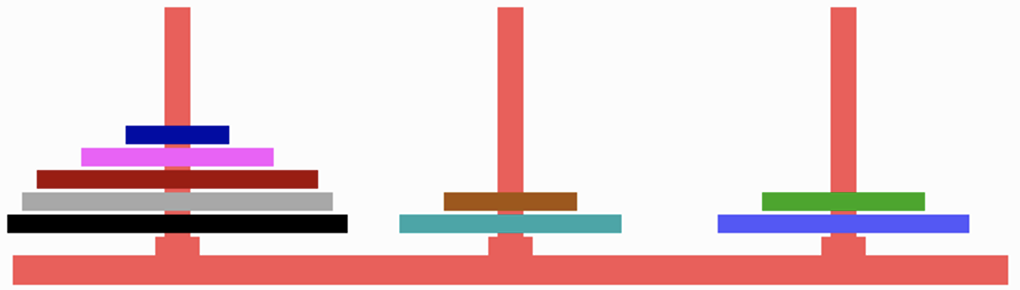
\includegraphics[scale=0.25]{hanoi.png} 
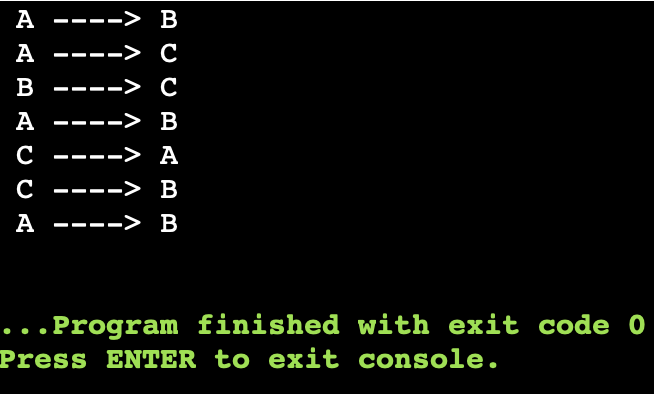
\includegraphics[scale=0.4]{hanoi2.png} 
\end{multicols}
\end{frame}
%%%%%%%%%%%%%%%%%%%%%%%%%%%%%%%%%%%%%%%%%%%%%%%%%%%%%%%%%%%%%%%%%

\begin{frame}[fragile]
\frametitle{Fonction récursive ;coût de Tour-de-Hanoï}
\begin{multicols}{2}
\begin{minted}[
%frame=lines,
framesep=2mm,
baselinestretch=1.2,
bgcolor=LightGray,
fontsize=\footnotesize,
% linenos
]{c}  
#include <stdio.h>
unsigned long c(int n){
    if(n==1) return 1;
    else return 2*c(n-1)+1;
}
int main(){ 
    int i;
    for(i=1;i<30;i++)
        printf("%ld ",c(i));
    return 0; 
}
\end{minted}
\\

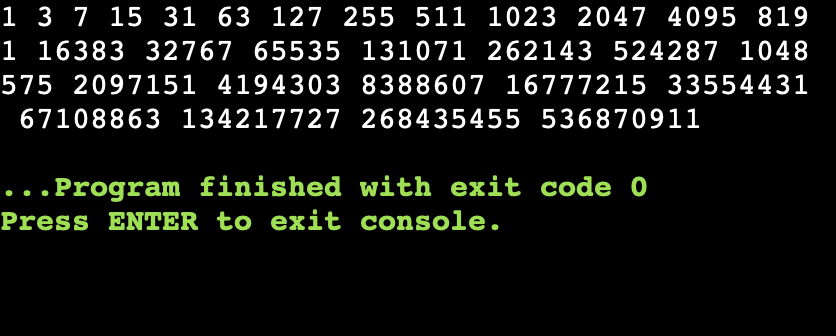
\includegraphics[scale=0.4]{hanoi3.png} 
\end{multicols}
\end{frame}
\end{document}

